\section{Einleitung}

\begin{frame}[t]
    \frametitle{Einleitung}
    
      \begin{columns}[t]
      \column[]{7cm}
      
      \begin{itemize}
      \item Mobile Roboter besitzen unterschiedliche Sensorsysteme
%       \begin{itemize}
%        \item RGB-Kameras
%        \item RGB-D-Kameras
%        \item Stereo-Kameras
%        \item 2D/3D Laserscanner
%       \end{itemize}
      \item Verschiedene Sensoren $\rightarrow$ verschiedene Eigenschaften
      \item Umgebungsmodellierung basierend auf unterschiedlichen Sensoren
      \end{itemize}
     

      \column{5cm}
      
      \begin{figure}[h]
	\centering
	    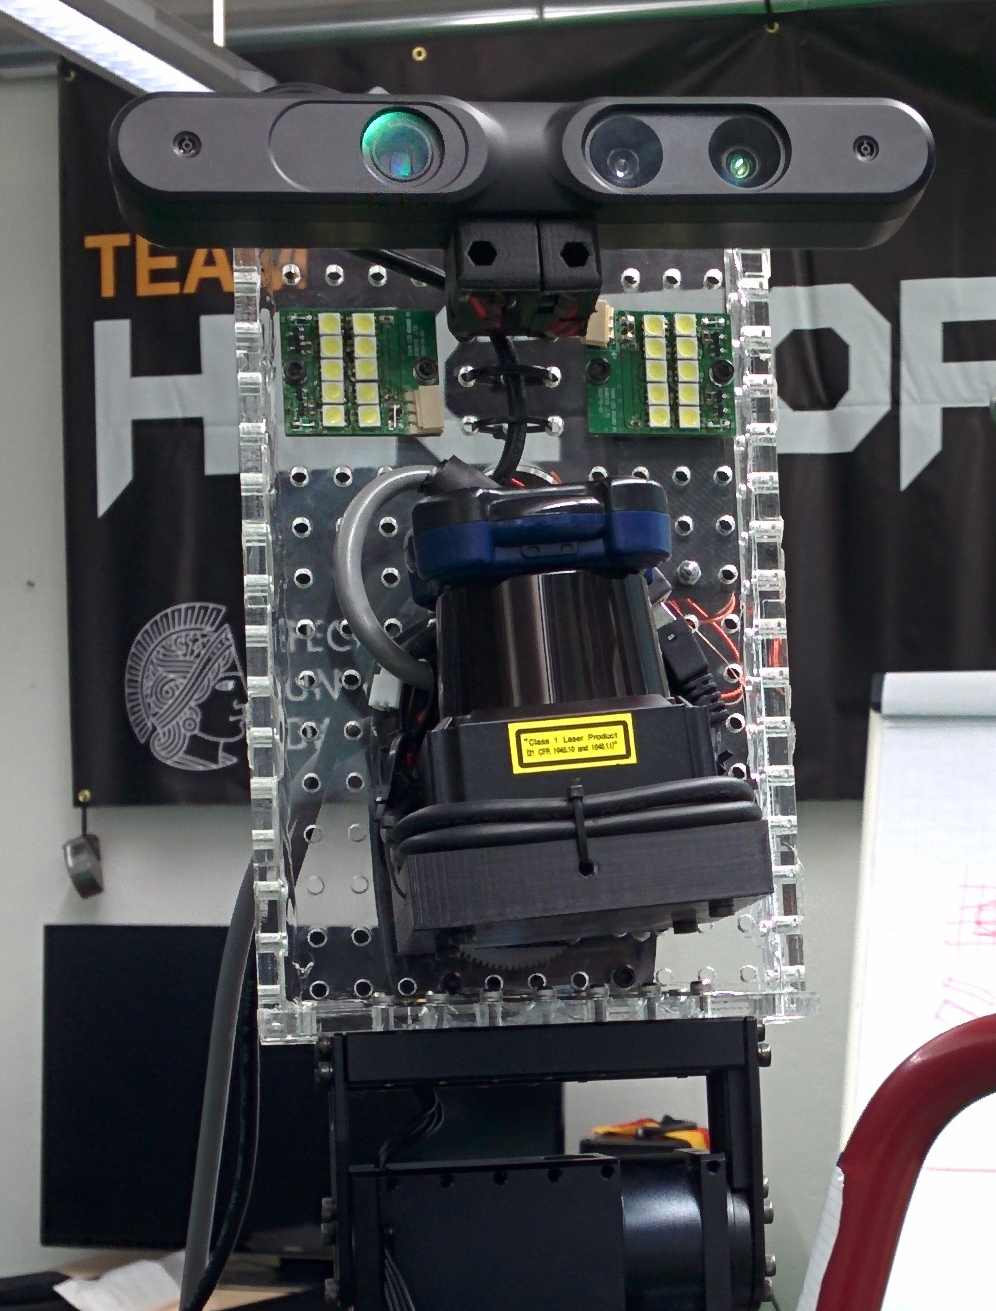
\includegraphics[width=3.5cm]{images/kopf}
	\caption{THOR-OPs Sensorkopf} 
      \end{figure}
  
    \end{columns}


\end{frame}


\subsection*{Motivation für Sensorfusions-Framework}
\begin{frame}[t]
    \frametitle{Motivation für Sensorfusions-Framework}

    \begin{itemize}
      \item Stärken von Sensoren kombinieren
      \item Schwächen ausmerzen
      \item Bestätigung der Daten von anderen Sensoren
      \item Verbesserung der Zuverlässigkeit der Umgebungsmodellierung
      \item Möglichkeiten eines guten (3D-) Weltmodells
      \begin{itemize}
	\item Fußschrittplanung
	\item Kollisionsvermeidung
	\item Pfadplanung
	\item Manipulationsaufgaben
	%\item Immersion bei Fernsteuerung
      \end{itemize}

\end{itemize}
\end{frame}


\subsection*{Anforderungen für Sensorfusions-Framework}






\begin{frame}[t]
  \frametitle{Anforderungen für Sensorfusions-Framework}
      
  \begin{itemize}
      \item Unterstützung beliebig vieler Sensoren
      \item Modellierung der Roboter-Umgebung 
      \item "`Echtzeit"'-Aktualisierungen
      \item Generierung von verschiedenen Umgebungsrepräsentationen
%       \begin{itemize}
% 	\item Höhenkarte
% 	\item Oberflächennormalen-Schätzung
%       \end{itemize}

      \item Effiziente CPU- und Speichernutzung
      \item Anwendbar für verschiedene Roboter und Sensorkonfigurationen
      \item ROS-Integration
  \end{itemize}

     

\end{frame}    




